\documentclass{article}
% Copyright 2017 Sergei Tikhomirov, MIT License
% https://github.com/s-tikhomirov/solidity-latex-highlighting/

\usepackage{listings, xcolor}

\definecolor{verylightgray}{rgb}{.97,.97,.97}

\lstdefinelanguage{Solidity}{
	keywords=[1]{anonymous, assembly, assert, balance, break, call, callcode, case, catch, class, constant, continue, constructor, contract, debugger, default, delegatecall, delete, do, else, emit, event, experimental, export, external, false, finally, for, function, gas, if, implements, import, in, indexed, instanceof, interface, internal, is, length, library, log0, log1, log2, log3, log4, memory, modifier, new, payable, pragma, private, protected, public, pure, push, require, return, returns, revert, selfdestruct, send, solidity, storage, struct, suicide, super, switch, then, this, throw, transfer, true, try, typeof, using, value, view, while, with, addmod, ecrecover, keccak256, mulmod, ripemd160, sha256, sha3}, % generic keywords including crypto operations
	keywordstyle=[1]\color{blue}\bfseries,
	keywords=[2]{address, bool, byte, bytes, bytes1, bytes2, bytes3, bytes4, bytes5, bytes6, bytes7, bytes8, bytes9, bytes10, bytes11, bytes12, bytes13, bytes14, bytes15, bytes16, bytes17, bytes18, bytes19, bytes20, bytes21, bytes22, bytes23, bytes24, bytes25, bytes26, bytes27, bytes28, bytes29, bytes30, bytes31, bytes32, enum, int, int8, int16, int24, int32, int40, int48, int56, int64, int72, int80, int88, int96, int104, int112, int120, int128, int136, int144, int152, int160, int168, int176, int184, int192, int200, int208, int216, int224, int232, int240, int248, int256, mapping, string, uint, uint8, uint16, uint24, uint32, uint40, uint48, uint56, uint64, uint72, uint80, uint88, uint96, uint104, uint112, uint120, uint128, uint136, uint144, uint152, uint160, uint168, uint176, uint184, uint192, uint200, uint208, uint216, uint224, uint232, uint240, uint248, uint256, var, void, ether, finney, szabo, wei, days, hours, minutes, seconds, weeks, years},	% types; money and time units
	keywordstyle=[2]\color{teal}\bfseries,
	keywords=[3]{block, blockhash, coinbase, difficulty, gaslimit, number, timestamp, msg, data, gas, sender, sig, value, now, tx, gasprice, origin},	% environment variables
	keywordstyle=[3]\color{violet}\bfseries,
	identifierstyle=\color{black},
	sensitive=true,
	comment=[l]{//},
	morecomment=[s]{/*}{*/},
	commentstyle=\color{gray}\ttfamily,
	stringstyle=\color{red}\ttfamily,
	morestring=[b]',
	morestring=[b]"
}

\lstset{
	language=Solidity,
	backgroundcolor=\color{verylightgray},
	extendedchars=true,
	basicstyle=\footnotesize\ttfamily,
	showstringspaces=false,
	showspaces=false,
	numbers=left,
	numberstyle=\footnotesize,
	numbersep=9pt,
	tabsize=2,
	breaklines=true,
	showtabs=false,
	captionpos=b
}
\usepackage{graphicx}


\title{Permissive Whitepaper}
\author{Flydexo, Philip}

\begin{document}
\maketitle
\begin{abstract}
    Our startup is developing an Account Abstraction EIP 4337 for permission-based authentication on the blockchain. This solution aims to simplify the process of managing permissions for smart contract interactions by enabling users to easily set up and manage permissions for all their interactions in a single gasless transaction. This will improve security on the blockchain and provide a more streamlined and user-friendly experience. Our solution will be particularly useful for DeFi newcomers and businesses and organizations that require a high level of security and control over their blockchain transactions.
\end{abstract}
\tableofcontents
\section{Motivation}
\paragraph{}
The Ethereum network has revolutionized the world of blockchain technology by providing a decentralized platform for secure and transparent transactions. However, managing permissions for smart contract interactions on the Ethereum network is still a challenge, with the current process being complex and time-consuming. Our startup aims to address this challenge by developing an Account Abstraction EIP 4337 for permission-based authentication on the Ethereum network.
\paragraph{}
With our solution, users will be able to easily manage permissions for all their smart contract interactions on the Ethereum network in a single transaction. By defining and enforcing permissions on their accounts, users can easily control which contracts they can interact with and which ones they cannot. This will improve security on the Ethereum network, reduce the risk of unauthorized access, and provide a more streamlined and user-friendly experience.
\paragraph{}
Our solution will be particularly useful for businesses and organizations that require a high level of security and control over their Ethereum transactions. By simplifying the process of managing permissions, our solution will enable these entities to conduct transactions more efficiently and securely, thereby saving time and reducing costs.
\paragraph{}
In conclusion, our startup is committed to improving the efficiency and security of the Ethereum network by developing an Account Abstraction EIP 4337 for permission-based authentication. We believe that our solution will be a game-changer in the world of Ethereum blockchain, enabling users to easily set up and manage permissions for all their smart contract interactions in a single transaction, and we are dedicated to bringing this innovation to the market.
\section{Business Model}
\paragraph{}
At Permissive, we strongly believe in the potential of open-source software to drive innovation. That is why our Permissive stack is built entirely on open-source technology and governed by the GNU General Public License v3.0. We believe that the codebase of Permissive contracts should be a public good, accessible to anyone who wishes to use or build upon it, whether they are an individual user, developer, or company.
\paragraph{}
However, our focus doesn't stop there. At Permissive, we recognize the importance of providing a great user experience to onboard the next billion users to the blockchain world. That's why we invest heavily in the design and usability of our platform. By providing an intuitive interface, we aim to make blockchain technology accessible to a wider audience, ultimately driving adoption and innovation.
\paragraph{}
To support our mission and cover the costs of platform development, we monetize through a small transaction fee. Every time a user initiates a transaction using the Permissive interface, a small fee of 0.01$-0.005$ is charged to their account. This fee allows us to continue developing and improving our platform, and it aligns with our values of accessibility and affordability.
\paragraph{}
Permissive plans to develop a complete ecosystem for blockchain. This ecosystem will include innovative tools and resources to simplify the blockchain experience for users and developers, driving greater adoption and innovation.
\section{Infrastructure}
\paragraph{}
The Permissive stack is designed to provide a seamless and secure user experience by utilizing both on-chain and off-chain computation. This approach allows for greater flexibility in the types of transactions that can be executed on the network, while also ensuring that users can engage with the platform safely and reliably. With the Permissive stack, users can enjoy the benefits of decentralized technology without having to worry about the complexities associated with traditional blockchain networks. Whether you are a developer looking to build decentralized applications or an end user seeking a more secure and efficient way to transact, the Permissive stack has something to offer. 
\subsection{On-Chain}
\paragraph{}
As Permissive is based on the EIP-4337 it can deploy on any EVM chain supporting it. We will first deploy on the most used EVM  and EIP-4337 compatible blockchains like Ethereum, Arbitrum, Optimism, Polygon, BNB Chain, Gnosis Chain, Avalanche, and Fantom. We also plan to build on new ecosystems like Base to onboard a larger user base.
\paragraph{}
Multiple contracts are required to make the Permissive function aligned with the EIP-4337 specifications. First, the PermissiveAccount, which is the main contract implements all the logic of Permissive. This contract exposes one function specific to Permissive and inherits from the Eth-Infitimism implementation and the ERC-4337 Interface. To store permissions efficiently, Permissive stores them in a Merkle root. This means that it will always take 32 bytes to store an infinite amount of permissions. Each operator is linked to a permission Merkle root and to a max fee and value authorization.
\begin{lstlisting}[language=Solidity]
struct Permission {
    // the operator
    address operator;
    // the address allowed to interact with
    address to;
    // the function selector
    bytes4 selector;
    // specific arguments that are allowed for this permission (see readme)
    // bytes allowed_arguments;
		// if set, the paymaster will be in charge of paying the fees
    address paymaster;
    // the timestamp when the permission isn't valid anymore
    // @dev can be 0 if expires_at_block != 0
    uint256 expiresAtUnix;
    // the block when the permission isn't valid anymore
    // @dev can be 0 if expires_at_unix != 0
    uint256 expiresAtBlock;
}

interface IAccount {
    function validateUserOp(UserOperation calldata userOp, bytes32 userOpHash, uint256 missingAccountFunds)
    external returns (uint256 validationData);
}

abstract contract BaseAccount is IAccount {
    using UserOperationLib for UserOperation;

    uint256 constant internal SIG_VALIDATION_FAILED = 1;

    function nonce() public view virtual returns (uint256);

    function entryPoint() public view virtual returns (IEntryPoint);

    function validateUserOp(UserOperation calldata userOp, bytes32 userOpHash, uint256 missingAccountFunds)
    external override virtual returns (uint256 validationData) {
        _requireFromEntryPoint();
        validationData = _validateSignature(userOp, userOpHash);
        if (userOp.initCode.length == 0) {
            _validateAndUpdateNonce(userOp);
        }
        _payPrefund(missingAccountFunds);
    }

    function _requireFromEntryPoint() internal virtual view {
        require(msg.sender == address(entryPoint()), "account: not from EntryPoint");
    }

    function _validateSignature(UserOperation calldata userOp, bytes32 userOpHash)
    internal virtual returns (uint256 validationData);

    function _validateAndUpdateNonce(UserOperation calldata userOp) internal virtual;

    function _payPrefund(uint256 missingAccountFunds) internal virtual {
        if (missingAccountFunds != 0) {
            (bool success,) = payable(msg.sender).call{value : missingAccountFunds, gas : type(uint256).max}("");
            (success);
        }
    }
}

interface IPermissiveAccount is IAccount {
    error InvalidProof();
    error NotAllowed(address);
    error InvalidTo(address provided, address expected);
    error ExceededValue(uint256 value, uint256 max);
    error ExceededFees(uint256 fee, uint256 maxFee);
    error InvalidPermission();
    error InvalidPaymaster(address provided, address expected);
    error InvalidSelector(bytes4 provided, bytes4 expected);
    error ExpiredPermission(uint current, uint expiredAt);

    event OperatorMutated(
        address operator,
        bytes32 oldPermissions,
        bytes32 newPermissions
    );

		function initialize(address owner) external;

    function setOperatorPermissions(
        address operator,
        bytes32 merkleRootPermissions,
        uint256 maxValue,
        uint256 maxFee
    ) external;
}
\end{lstlisting}
\paragraph{}
Permissive has a custom factory for deploying Permissive Accounts directly with a user operation off-chain.
\subsection{WebApp}
The Permissive app is composed of three main pages. The Operator, Authorization and Account page. The operator page is where the service or user wants to get permission over someone’s else address. To do so, the interface will allow him to create permissions sets and format them for blockchain compatibility. Once the Merkle root is computed, the app stores the permissions into IPNS with the corresponding Merkle root. Once done, the operator can copy the authorization URL to send it to the user.  The authorization page is the page where the user can see the permissions the operator wants on its account and grant them or not. (similar to web2 AUTH systems). Finally, the Account page is where the user can see all the permissions he has granted, revoke them or add increase their maximum fees or value.
\subsection{CallData}
\paragraph{}
t the time of writing this whitepaper, function arguments are not verified against user permissions. This means that anyone can execute a function regardless of whether they have the necessary permissions or not. This could lead to security vulnerabilities and potential abuse of the system.
\paragraph{}
To tackle this issue, we are developing an allowance call data format that will allow for conditional and customizable arguments. This new format will enable us to verify user permissions before executing a function, ensuring that only authorized users can execute transactions that require specific permissions. As such, we will be releasing detailed documentation and a technical paper that outlines the allowance call data format and how it works.
\subsection{Plugins, Modules \& SDKs}
To ensure that Permissive is available to as many users as possible, regardless of their account type, we will be creating plugins for existing Account Abstraction solutions and development kits. These plugins will allow for the seamless integration of Permissive into a wide range of accounts, making it easy for users to take advantage of its many benefits. In addition, we will be working closely with developers to ensure that the plugins are easy to use and integrate, with clear documentation and support available at every step of the way. With these efforts, we aim to make Permissive a truly accessible and user-friendly platform for all.
\section{Workflow}
\begin{center}
    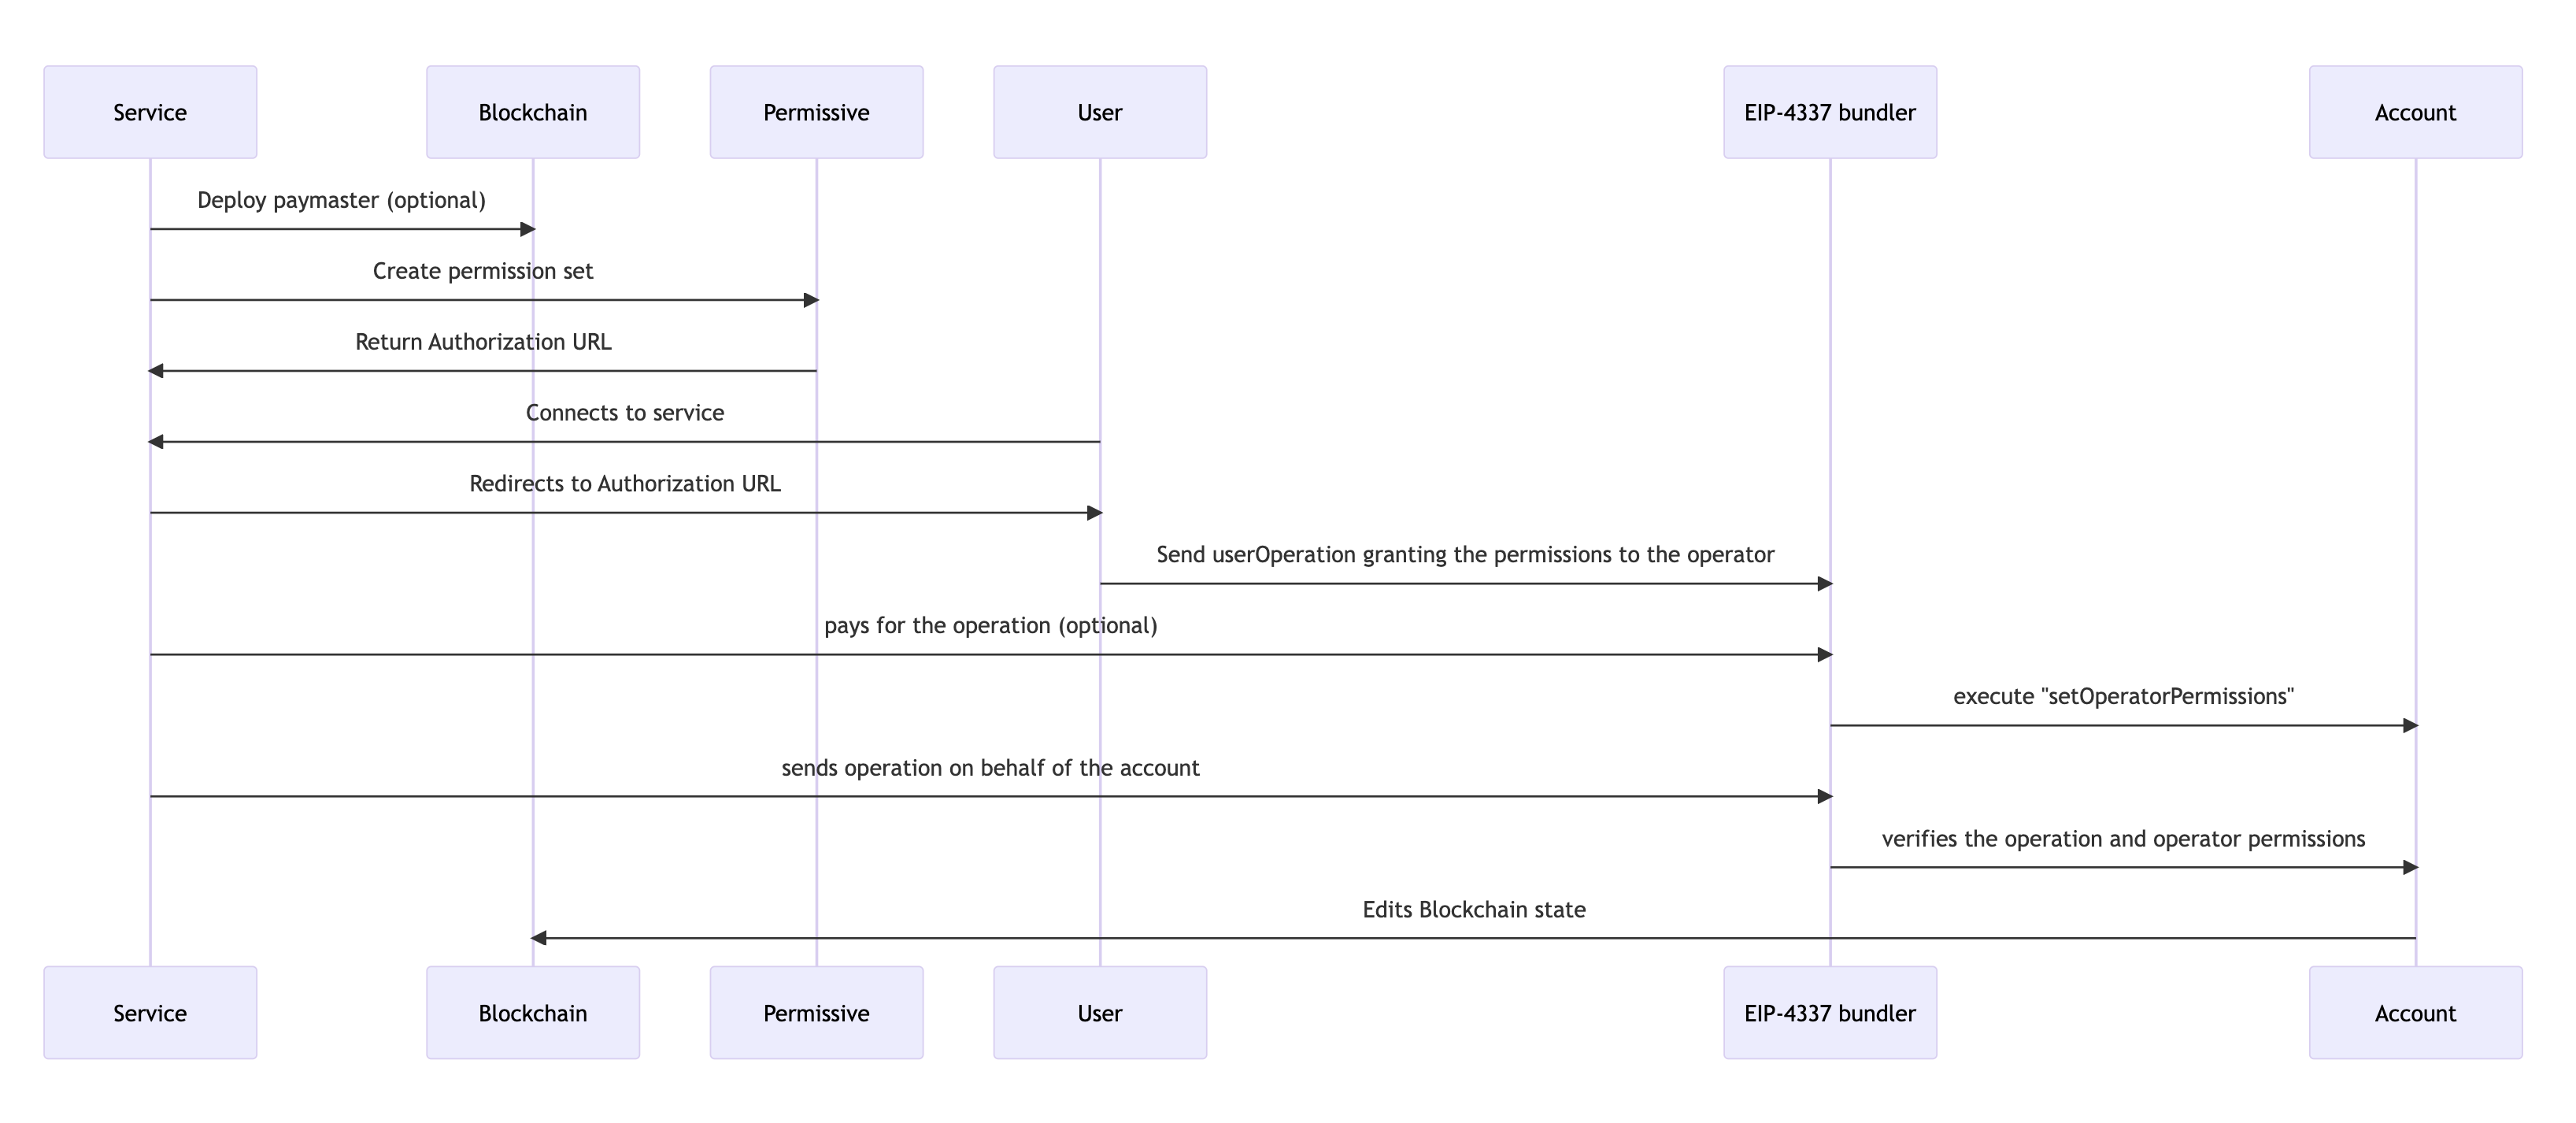
\includegraphics[scale=0.2]{schema.png}
\end{center}
\section{Roadmap}
The Permissive project is a comprehensive initiative that aims to go beyond its current focus on Account-Abstraction. Our goal is to expand the offerings and features of the project to enable developers, companies, and users to onboard the next set of users to the blockchain. We have a plan in place to release a complete SDK for both clients and servers to facilitate interaction with the Permissive protocol. This SDK will include a wide range of tools and capabilities, including an array of plugins and modules designed to take advantage of the best solutions in the ecosystem.
\paragraph{}
But that's not all. Our team is also working on a number of complementary products that will enhance the overall experience of using Permissive. These products include bundlers, nodes, paymasters, and more, all of which will work in harmony with the Permissive protocol to create a seamless and user-friendly platform.
\end{document}